%This is the first chapter of the dissertation

%The following command starts your chapter. If you want different titles used in your ToC and at the top of the page throughout the chapter, you can specify those values here. Since Columbia doesn't want extra information in the headers and footers, the "Top of Page Title" value won't actually appear.

\chapter[Results][Top of Page Title]{Title of Chapter 1}

Here you can write some introductory remarks about your chapter.
I like to give each sentence its own line.

When you need a new paragraph, just skip an extra line.

\section{Statistical Analysis}

maybe to be moved to an appendix

\section{Signal Region distributions}

\subsection{Scale variable distributions in the signal regions}

In \ref{fig:srs_scale,fig:srg_scale,fig:src_scale}, we can see the distributions of the last scale cut used for each signal region.
These distributions include scale factors derived via the fitting procedure which are applied to the Standard Model background, which we will describe later in this chapter.
These scale factors are all $\order 1$.
The systematic uncertainties, shown in the banded stripe, are also described later in this section.
Each plot shows the distribution from a signal model which is targetted by the given signal region.

These distributions have all cuts applied except for the cut on this scale variable, which allows us to see the additional discrimination provided by the given variable.
Since signal regions with the same numeral have identical cuts on all cuts other than the main scale variable, we show (a) and (b) on the same figure.
The left-most (right-most) arrow shown is the location of the a (b) cut applied in the analysis.
We call these plot \textit{$N-1$} plots, where $N$ refers to the number of cuts applied in the analysis.
The full set of $N-1$ plots in the signal regions for the other variables used in the analysis are shown in \ref{app:n-1_plots}.
We can see that for the signal models targeted by each signal region, each cut provides unique discrimination against the Standard Model backgrounds.

\begin{figure}[tbp]
\begin{center}
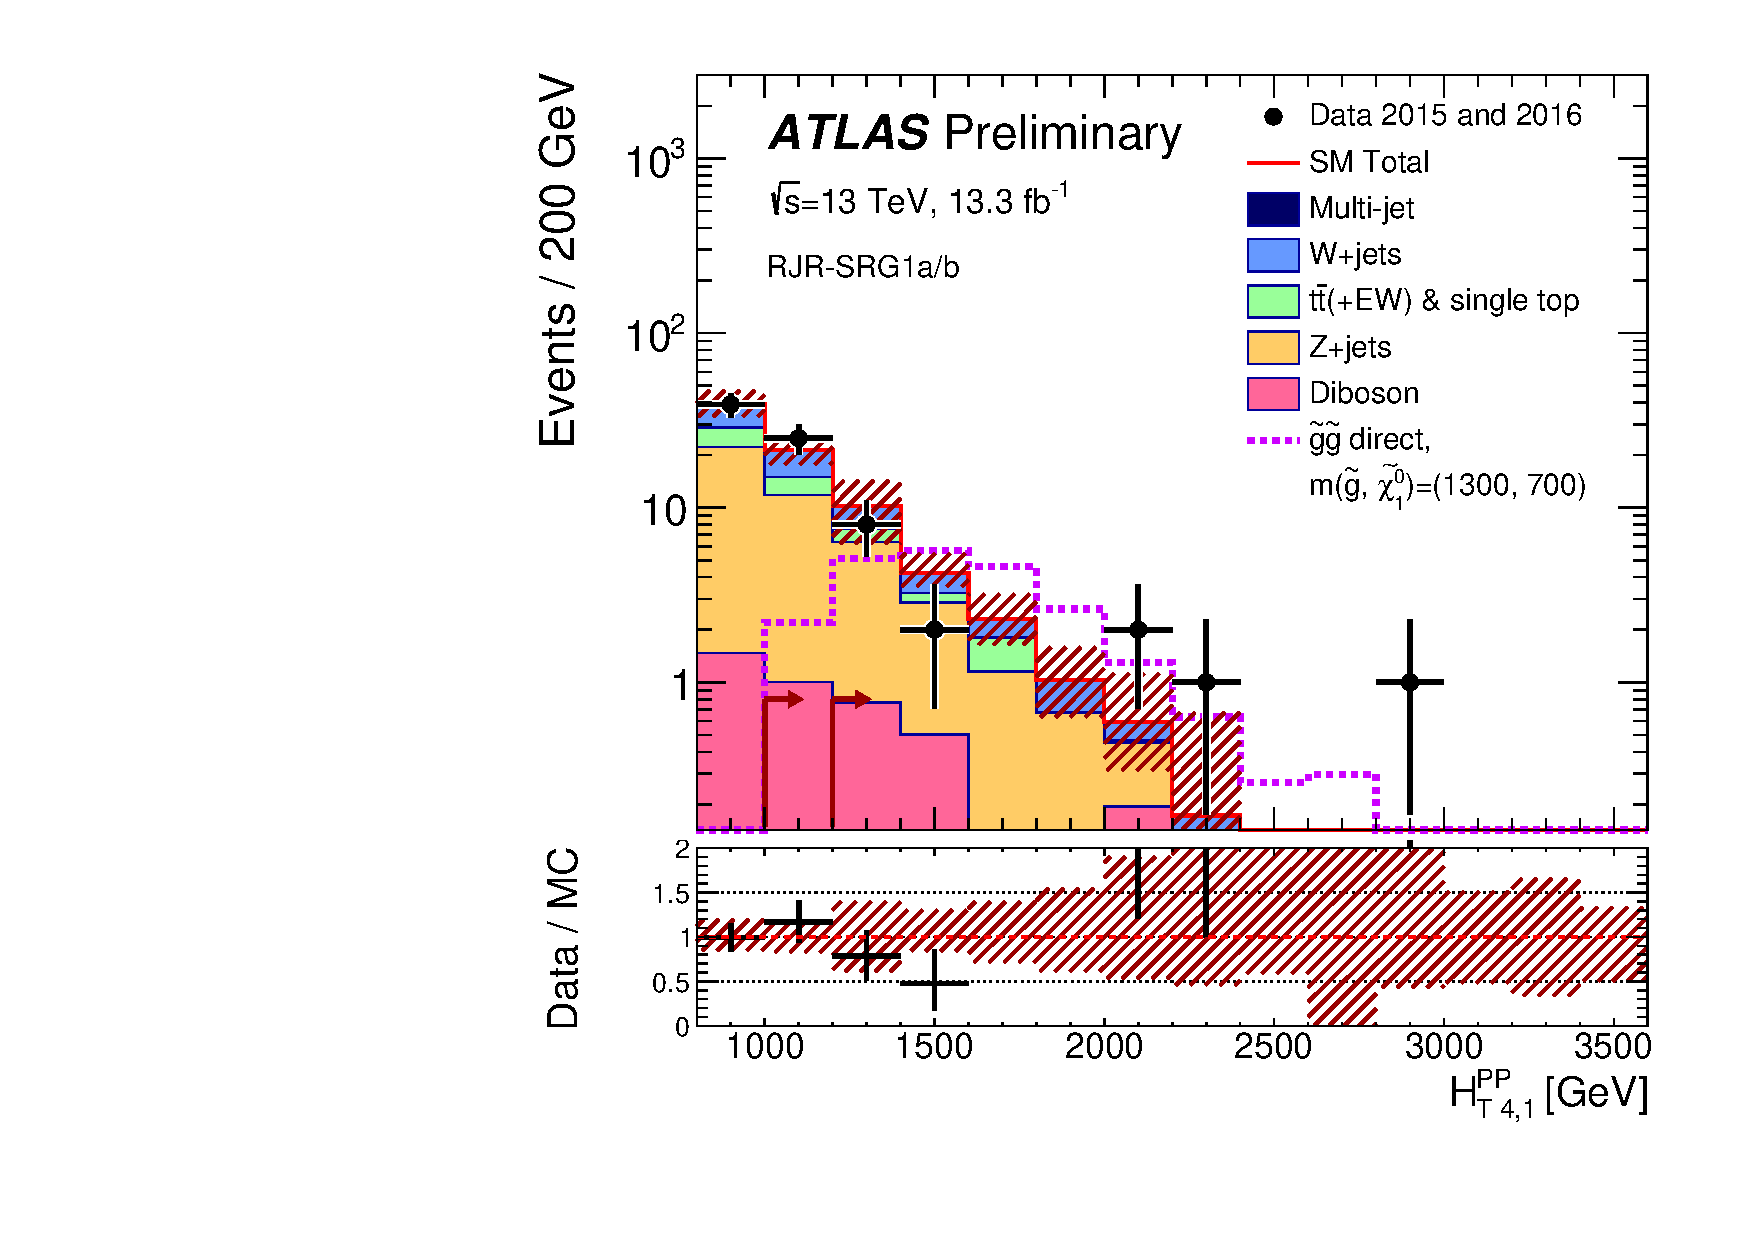
\includegraphics[width=0.45\textwidth]{ATLAS-CONF-2016-078_INT/N-1Plots/AtlasStyle/Preliminary/SR_SRJigsawSRG1a_LastCut_SR_minusone}
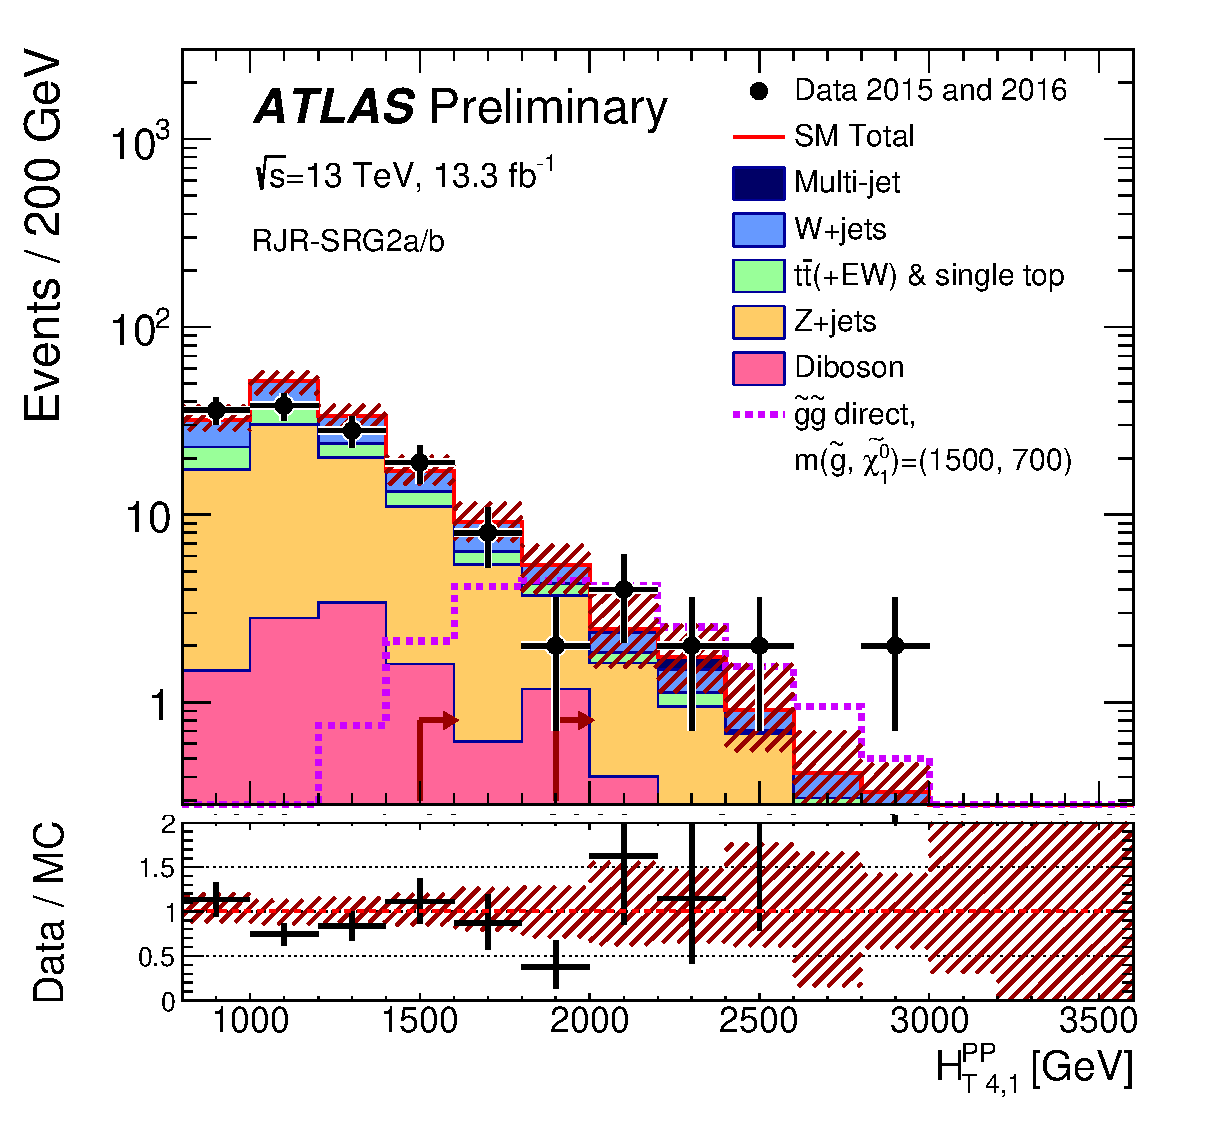
\includegraphics[width=0.45\textwidth]{ATLAS-CONF-2016-078_INT/N-1Plots/AtlasStyle/Preliminary/SR_SRJigsawSRG2a_LastCut_SR_minusone}
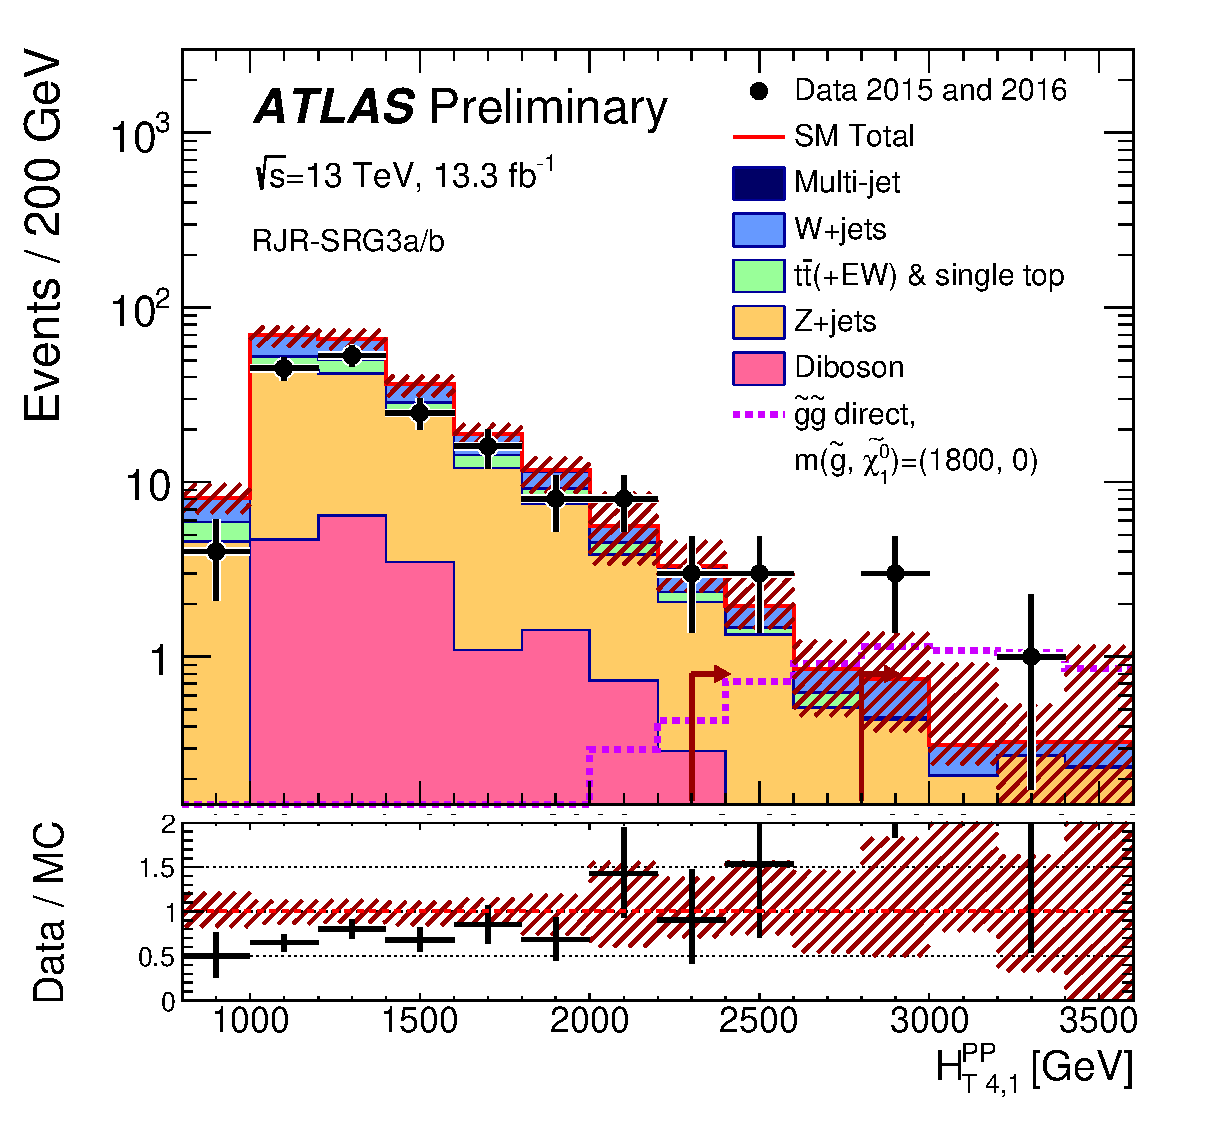
\includegraphics[width=0.45\textwidth]{ATLAS-CONF-2016-078_INT/N-1Plots/AtlasStyle/Preliminary/SR_SRJigsawSRG3a_LastCut_SR_minusone}
\end{center}
\caption{Scale variable distributions for the gluino signal regions.}
\label{fig:srg_scale}
\end{figure}

\begin{figure}[tbp]
\begin{center}
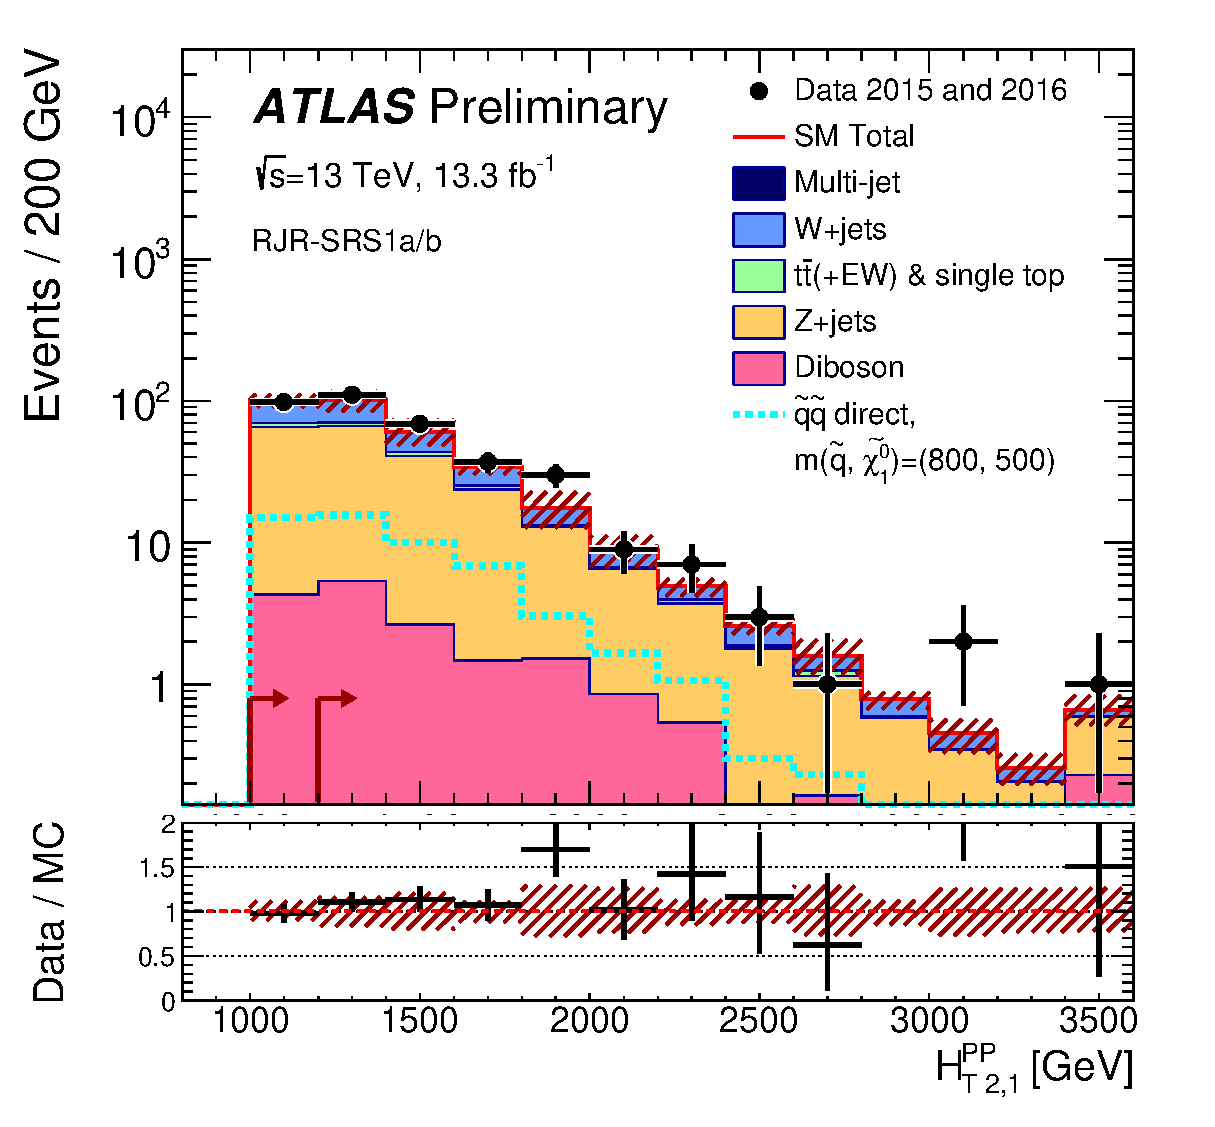
\includegraphics[width=0.45\textwidth]{ATLAS-CONF-2016-078_INT/N-1Plots/AtlasStyle/Preliminary/SR_SRJigsawSRS1a_LastCut_SR_minusone}
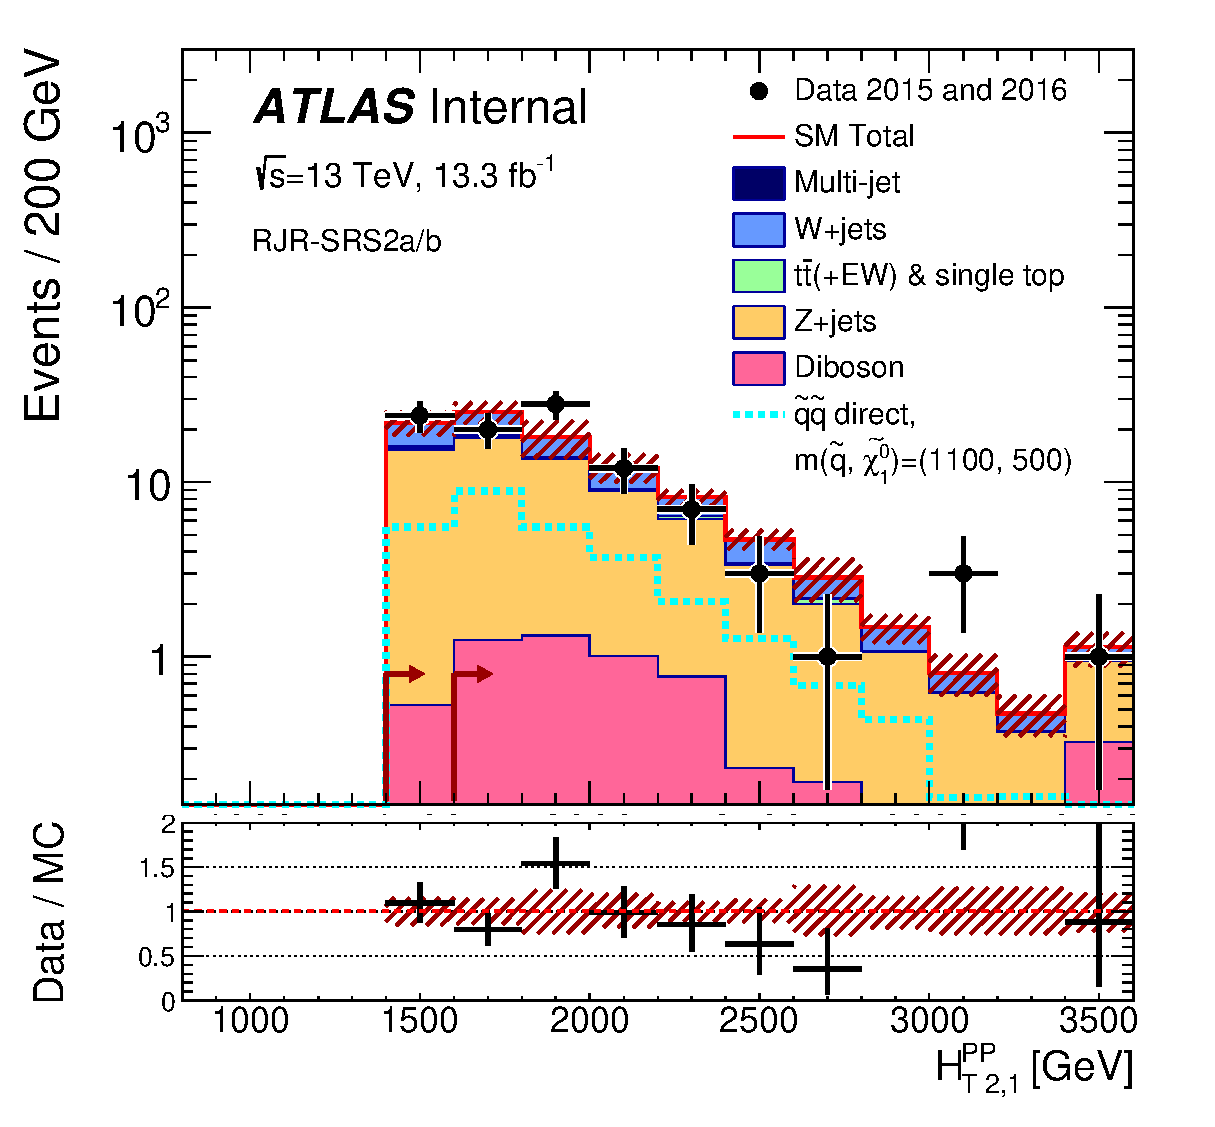
\includegraphics[width=0.45\textwidth]{ATLAS-CONF-2016-078_INT/N-1Plots/AtlasStyle/Preliminary/SR_SRJigsawSRS2a_LastCut_SR_minusone}
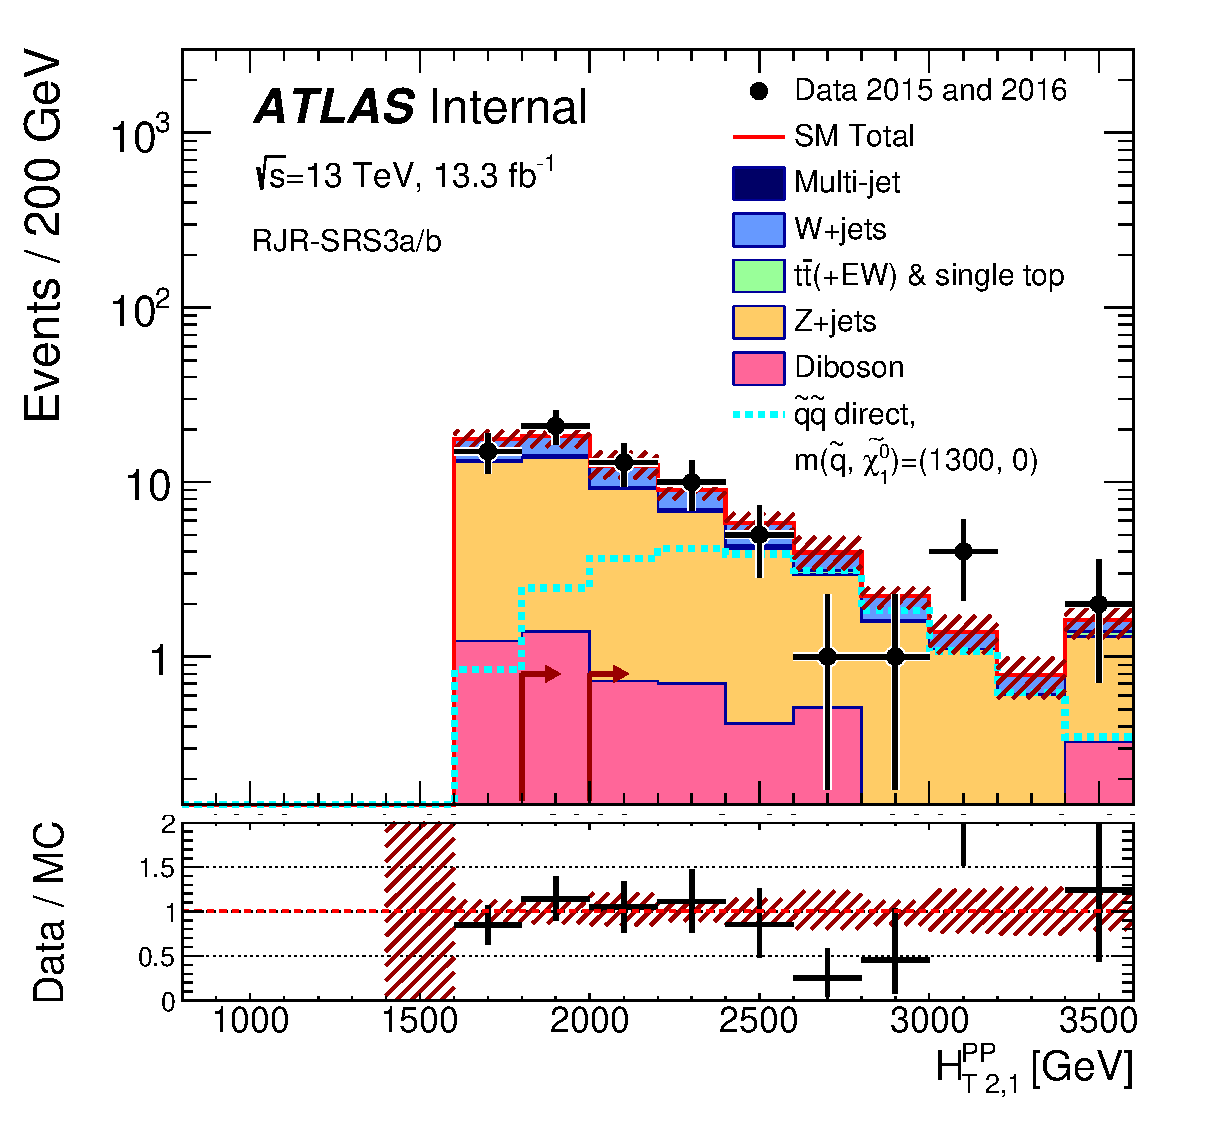
\includegraphics[width=0.45\textwidth]{ATLAS-CONF-2016-078_INT/N-1Plots/AtlasStyle/Preliminary/SR_SRJigsawSRS3a_LastCut_SR_minusone}
\end{center}
\caption{Scale variable distributions for the squark signal regions.}
\label{fig:srs_scale}
\end{figure}

\begin{figure}[tbp]
\begin{center}
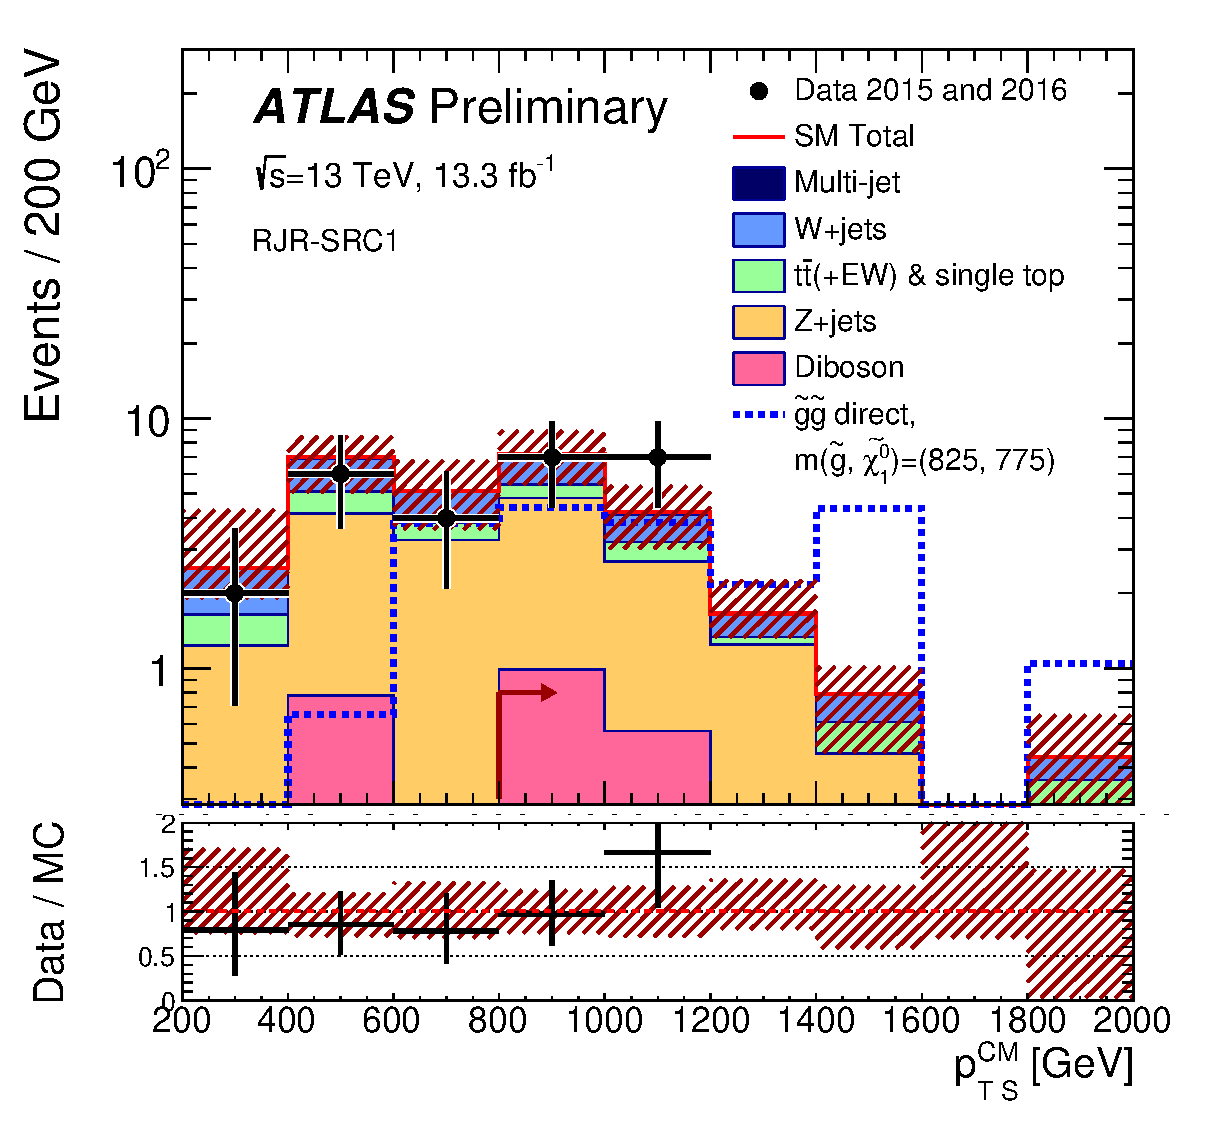
\includegraphics[width=0.45\textwidth]{ATLAS-CONF-2016-078_INT/N-1Plots/AtlasStyle/Preliminary/SR_SRJigsawSRC1_LastCut_SR_minusone}
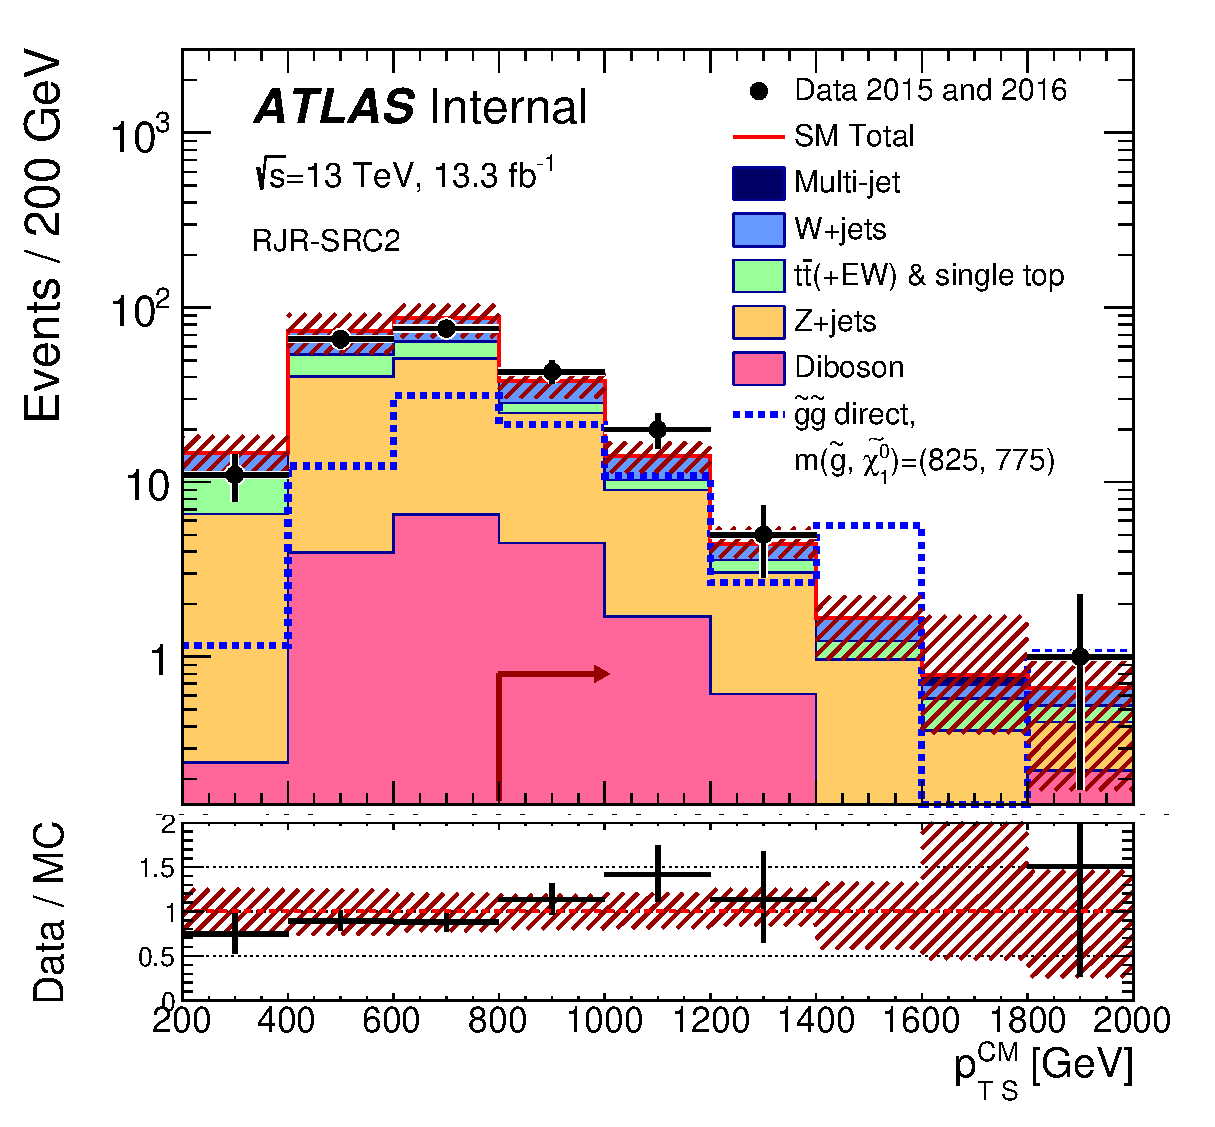
\includegraphics[width=0.45\textwidth]{ATLAS-CONF-2016-078_INT/N-1Plots/AtlasStyle/Preliminary/SR_SRJigsawSRC2_LastCut_SR_minusone}
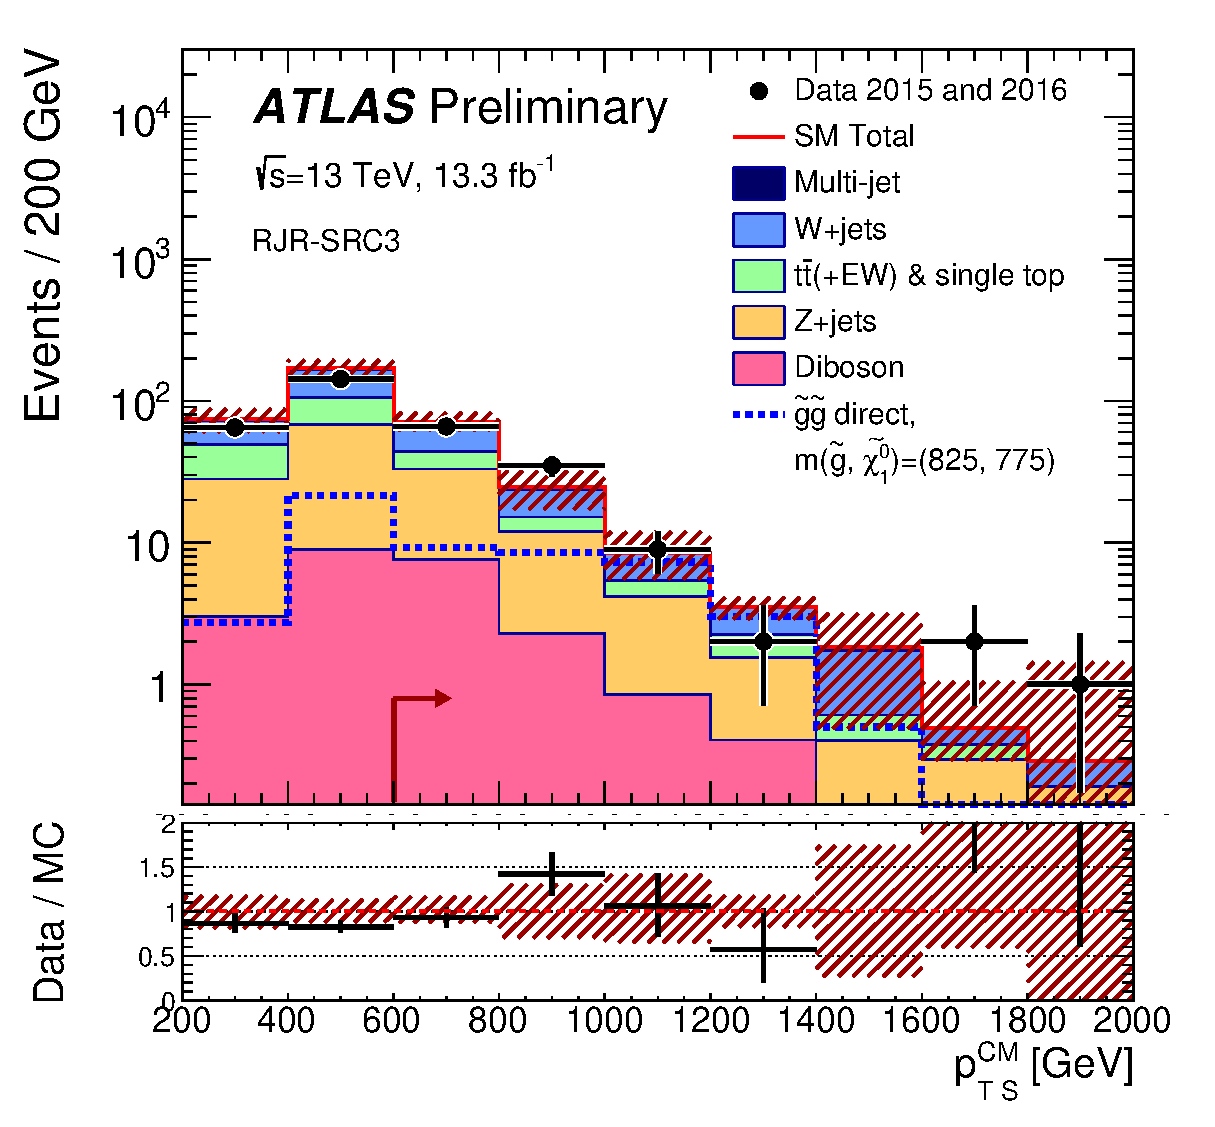
\includegraphics[width=0.45\textwidth]{ATLAS-CONF-2016-078_INT/N-1Plots/AtlasStyle/Preliminary/SR_SRJigsawSRC3_LastCut_SR_minusone}
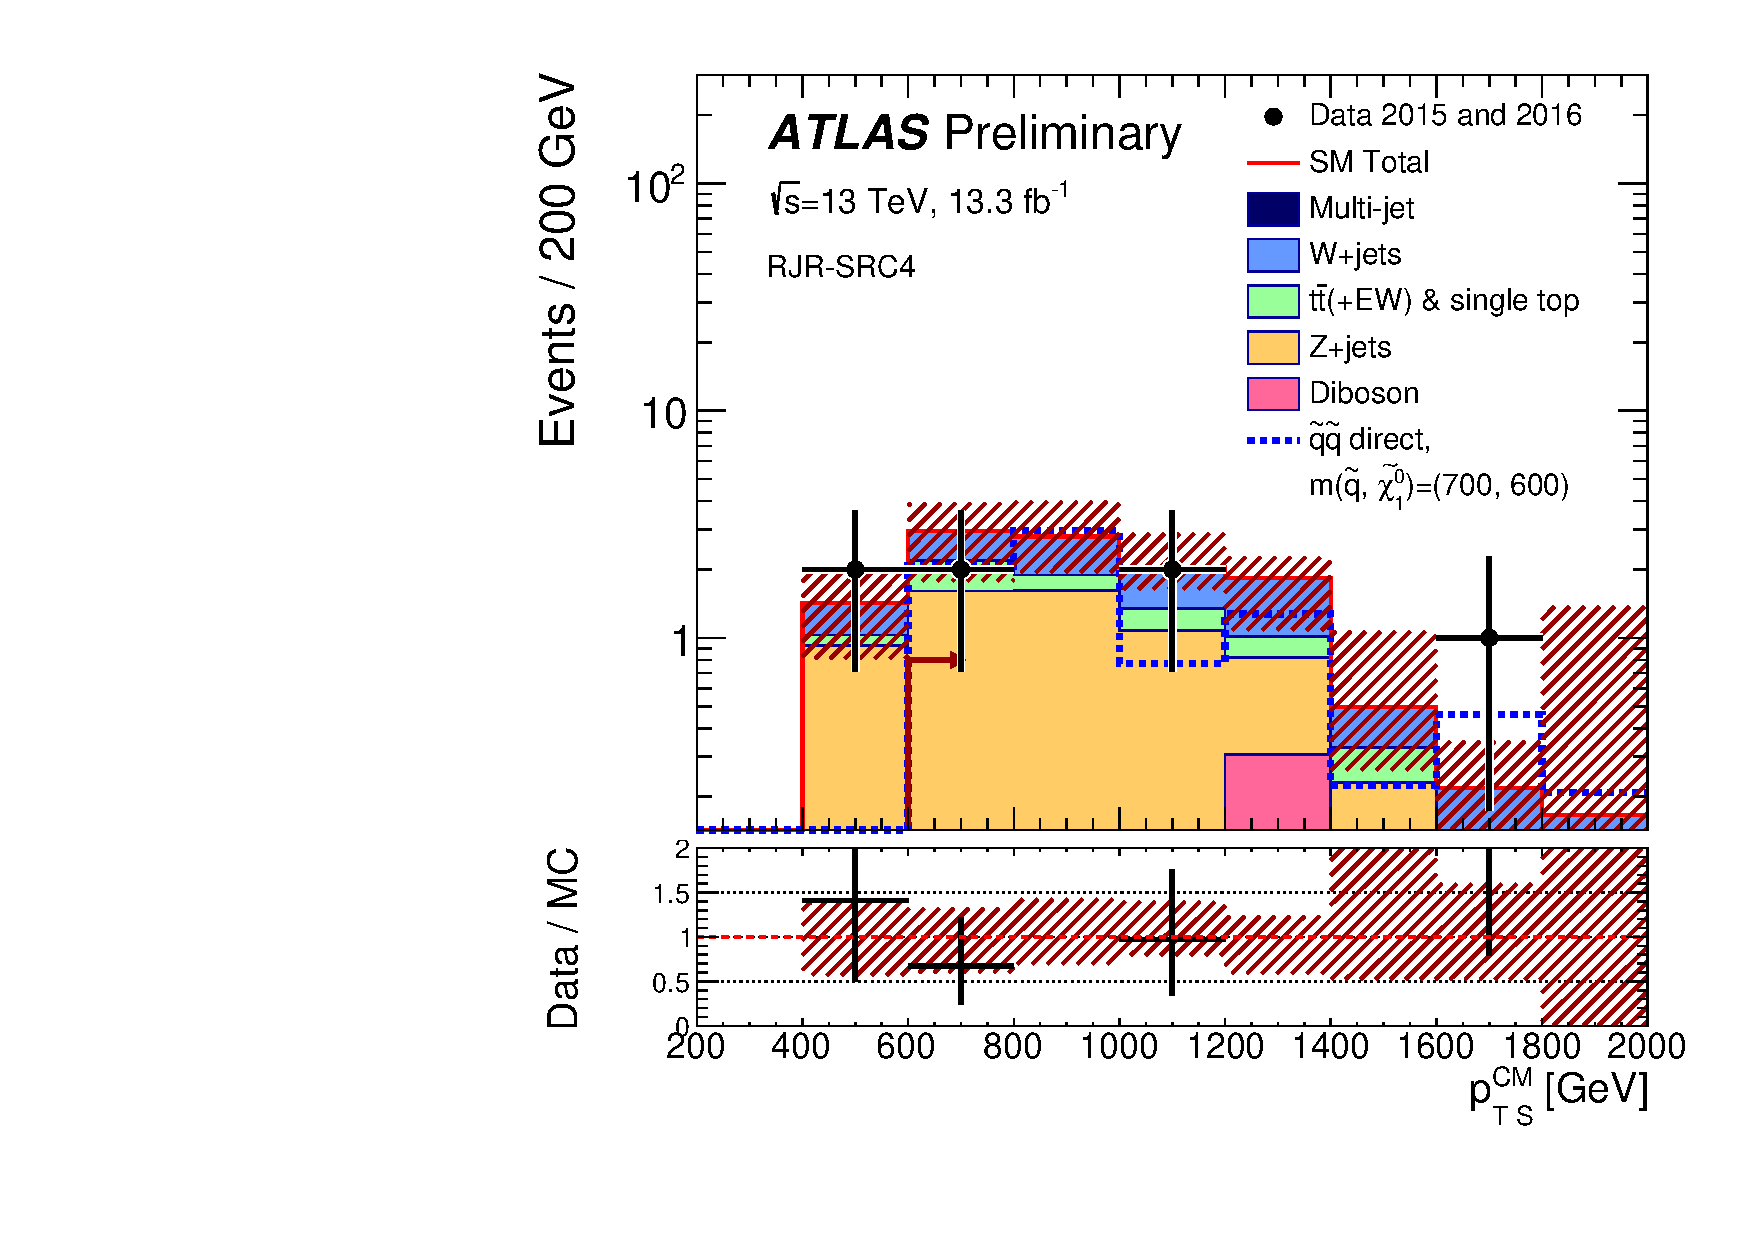
\includegraphics[width=0.45\textwidth]{ATLAS-CONF-2016-078_INT/N-1Plots/AtlasStyle/Preliminary/SR_SRJigsawSRC4_LastCut_SR_minusone}
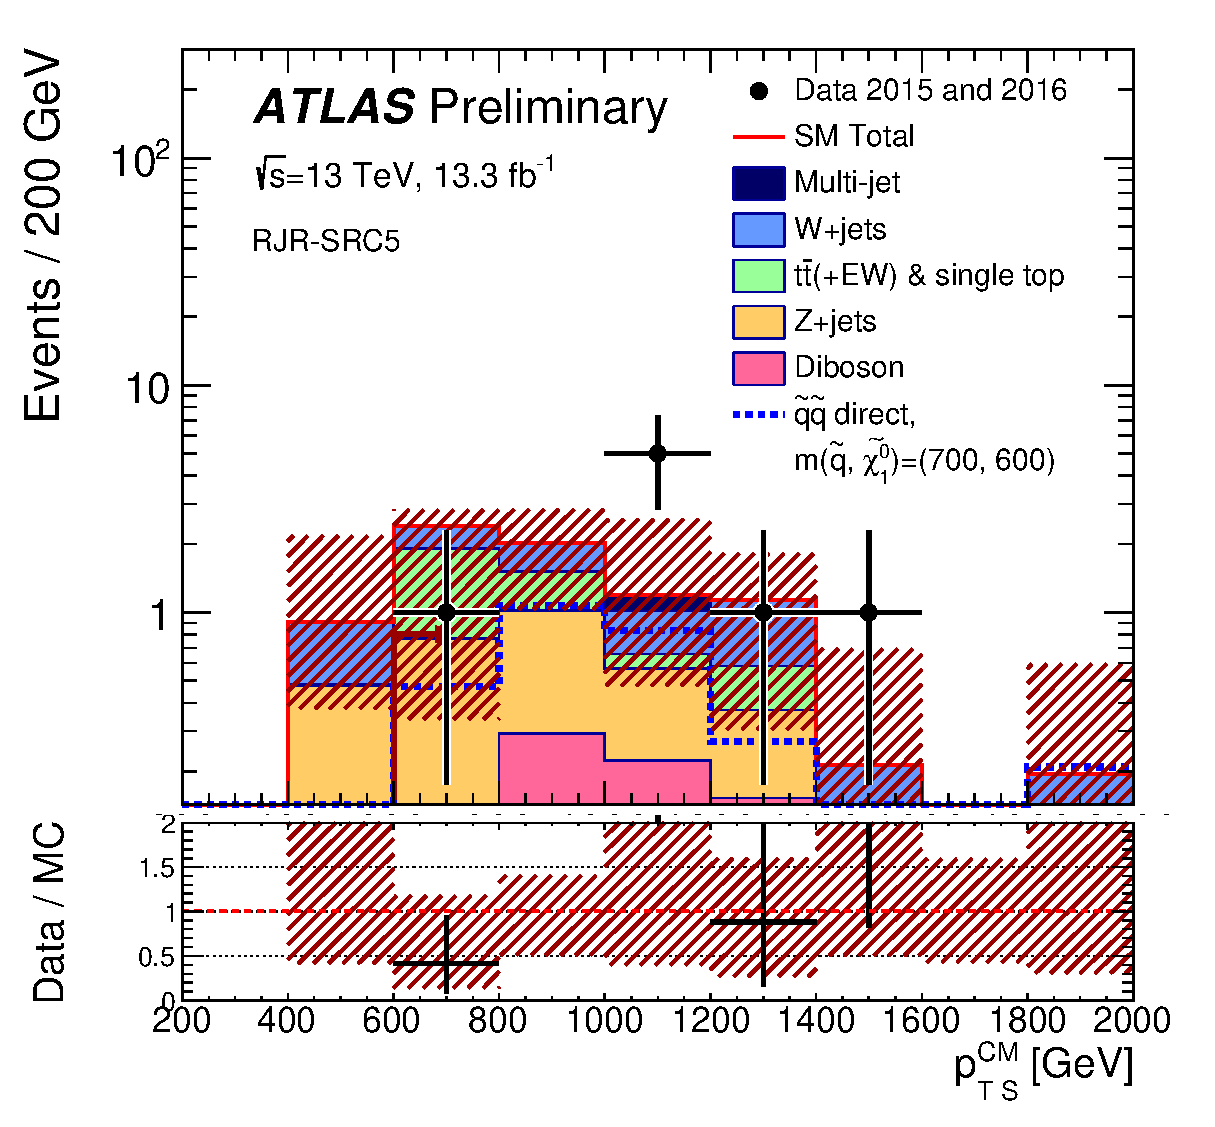
\includegraphics[width=0.45\textwidth]{ATLAS-CONF-2016-078_INT/N-1Plots/AtlasStyle/Preliminary/SR_SRJigsawSRC5_LastCut_SR_minusone}
\end{center}
\caption{Scale variable distributions for the compressed signal regions.}
\label{fig:src_scale}
\end{figure}



\section{Pull Plots}

\section{Exclusion plots}
